\documentclass[a4paper,12pt]{article}

\usepackage[utf8]{inputenc}
\usepackage[T1]{fontenc}
\usepackage{a4}
\usepackage{lipsum}
\usepackage{graphicx}
\usepackage{float}
\usepackage{listings}
\usepackage{color}
\usepackage{hyperref}
\usepackage{cite}
\usepackage{textgreek}
\usepackage{amsfonts}

\usepackage[margin=1in]{geometry}

\definecolor{dkgreen}{rgb}{0,0.6,0}
\definecolor{gray}{rgb}{0.5,0.5,0.5}
\definecolor{mauve}{rgb}{0.58,0,0.82}

\lstset{frame=tb,
  language=matlab,
  aboveskip=5mm,
  belowskip=5mm,
  showstringspaces=false,
  columns=flexible,
  basicstyle={\small\ttfamily},
  numberstyle=\tiny\color{gray},
  keywordstyle=\color{blue},
  commentstyle=\color{dkgreen},
  stringstyle=\color{mauve},
  breaklines=true,
  breakatwhitespace=true,
  tabsize=2
}

\title{
  {\Huge \bf Power Systems Lab}\\
  \vspace{0.25in}

  {\bf Experiment 5}\\
  Laboratory Report
  \vspace{1in}
}
\author{
  \bf Syed Alisamar Husain, 17BEE012\\
  B.Tech Electrical Engg, 8th Semester
}

\begin{document}
  \begin{titlepage}
    \maketitle
    \vspace*{\fill}
    \begin{center}
      {\bfseries Department of Electrical Engineering} \\
      Jamia Millia Islamia, New Delhi
    \end{center}
    \thispagestyle{empty}
  \end{titlepage}
  
  \newpage
  \begin{center}
    \huge Experiment 5
    \vspace{0.5in}
  \end{center}

  \section{Objective}
  To construct the V-curve for a synchronous motor with varying field excitation 
  from leading to lagging power factor assuming suitable open-circuit characteristics.

  Let the given problem be as follows:

  \section{Theoretical Background}
  {\bf V-curve} is a plot of the {\bf stator current versus field current} for different 
  constant loads. The graph plotted between the armature current $I_a$ and field 
  current $I_f$ at no load the curve is obtained known as V-Curve. Since the 
  shape of these curves is similar to the letter “V”, thus they are called the 
  V-curve of a synchronous motor.
  
    \begin{figure}[H]
      \centering
      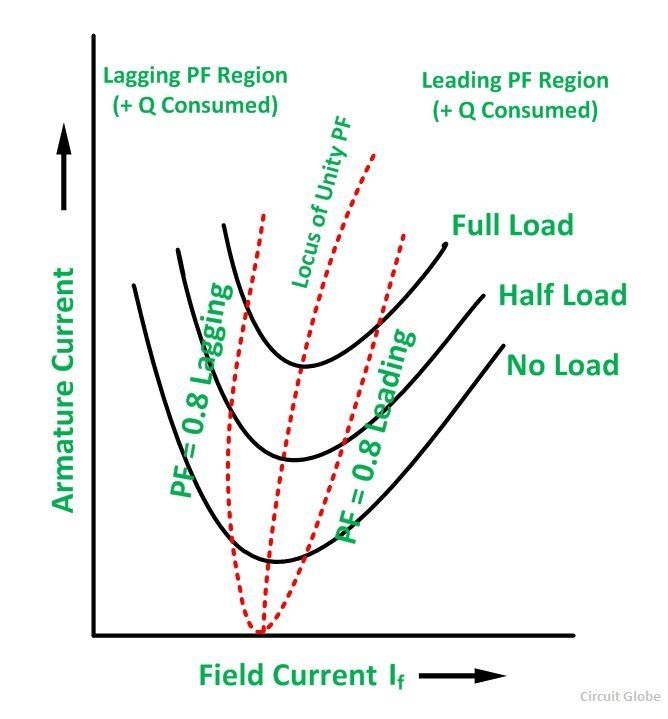
\includegraphics[width=3.5in]{img/vcurves.jpg}
      \label{vcurves}
      \caption{V-Curves of a Synchronous Motor}
    \end{figure}

    \subsection{Plotting a V-Curve}
    The power factor of the synchronous motor can be controlled by varying the 
    field current $I_f$. The armature current $I_a$ changes with the change 
    in the field current $I_f$. 
    
    Let us assume that the motor is running at no load. If the field current is increased 
    from this small value, the armature current $I_a$ decreases until the armature current 
    becomes minimum. At this minimum point, the motor is operating at a unity power factor. 
    The motor operates at a lagging power factor until it reaches up to this point of operation.

    If now, the field current is increased further, the armature current increases and 
    the motor starts operating as a leading power factor. 
    The graph drawn between armature current and field current is known as the V curve. 
    If this procedure is repeated for various increased loads, a family of curves is obtained.

    \subsection{Unity Power Factor Compounding Curve}
    The point at which the unity power factor occurs is at the point where the armature 
    current is minimum. {\bf The curve connecting the lowest points of all the V curves 
    for various power levels is called the Unity Power Factor Compounding Curve.}
    The compounding curves for 0.8 power factor lagging and 0.8 power factor leading 
    are shown in the figure above by a red dotted line.

    The loci of constant power factor points on the V curves are called Compounding 
    Curves. It shows the manner in which the field current should be varied in order 
    to maintain a constant power factor under changing load. Points on the right and 
    left of the unity power factor corresponds to the over-excitation and leading 
    current and under excitation and lagging current respectively.

  \pagebreak
  \section{Implementation}
  \begin{lstlisting}
    % To construct the V-curve for a synchronous motor with varying  
    % field excitation from leading to lagging power factor

    % 17BEE012 - Alisamar Husain

    If = (38:1:58) / 10;    % Field currents from 3.8 A to 5.8 A
    Ia = zeros(1,21);       % Armature currents to be calculated

    Xs = 2.5;               % Synchronous reactance

    Vp = 210;
    delta1 = -12 * (pi/180);

    Ea1 = 200 * (cos(delta1) + 1j*sin(delta1));

    % Calculate armature current for each value
    for i = (1:21)
        Ea2= 45.5 * If(i);
        
        delta2 = asin( (Ea1/Ea2) * sin(delta1) );
        Ea2 = Ea2 * (cos(delta2) + 1j*sin(delta2));
        
        Ia(i) = (Vp - Ea2) / (1j * Xs);
    end

    figure(1);
    plot(If, abs(Ia), 'Color', 'k', 'LineWidth', 2.0);
    xlabel('Field Current');
    ylabel('Armature Current');
    grid on;
  \end{lstlisting}

  \pagebreak
  \section{Observations}
  The following graph for the V-Curve of Synchronous Motor was obtained.
  {\bf Unity power factor} was obtained at 4.9 A of Field current where the Armature
  current was close to 15.8 A.
    \subsection{Graphs and Plots}
    \begin{figure}[H]
      \centering
      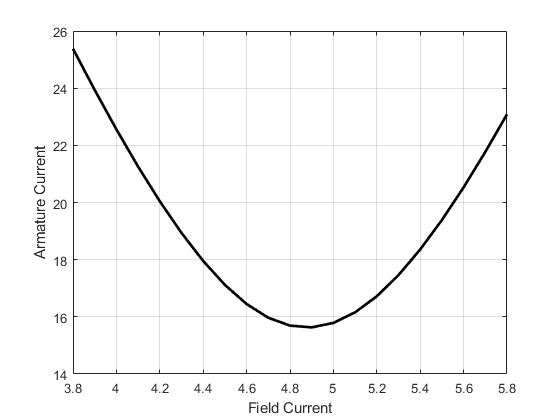
\includegraphics[width=5in]{img/vc2.png}
      \label{result}
      \caption{V-Curve of a Synchronous Motor}
    \end{figure}

  \section{Result}
  The V-curve graph was plotted between the armature current $I_a$ and field 
  current $I_f$ for a synchronous motor.

\end{document}